\section{Introduction}\label{sec:intro}

\IEEEPARstart{T}{he} rapid convergence of edge computing and multimodal artificial intelligence has catalyzed the deployment of edge-assisted Visual Question Answering (VQA) in mission-critical applications, ranging from autonomous unmanned aerial vehicle (UAV) reconnaissance to smart environmental monitoring and industrial robotic inspection~\cite{lobry2020rsvqa,zheng2024aerialee}. In these cyber-physical scenarios, a resource-constrained wireless edge transmitter captures high-resolution visual imagery and transmits visual data over band-limited, fading wireless uplinks to an edge computing node equipped with a foundational Vision--Language Model (VLM)~\cite{wang2024qwen2vl,bai2025qwen25vl}. By combining deep spatial perception with natural language reasoning, the edge VLM can provide accurate answers to diverse semantic queries.

However, executing high-fidelity VQA over real-world wireless networks faces two profound, interdependent resource bottlenecks that directly challenge the sustainability of green edge networks:
\begin{enumerate}
    \item \textbf{Wireless Channel Degradation and Physical Outage}: Conventional wireless links suffer from multipath fading, shadowing, and signal attenuation. Under standard bit-level separate source-channel coding (SSCC) and discrete block-length channel codes such as low-density parity-check (LDPC) codes, channel degradation leads to severe packet delivery outages (the ``cliff effect'')~\cite{bourtsoulatze2019djscc}. When transmission energy is strictly constrained, transmitting large uncompressed or lightly compressed bitstreams over degraded channels inevitably causes decoding failure and catastrophic answer errors.
    \item \textbf{Multimodal Token Explosion and Edge Computation Costs}: Modern autoregressive VLMs utilize visual tokenizers that project image patches into dense sequences of visual tokens~\cite{wang2024qwen2vl}. The computational complexity of the self-attention mechanism scales quadratically with the visual token count, $\mathcal{O}(T_v^2)$, where $T_v$ denotes the sequence length. Processing dense visual representations for simple, localized questions (e.g., verifying object presence) imposes severe computational and energy burdens on the edge server without offering tangible task-accuracy benefits.
\end{enumerate}

To overcome the spectral and energy inefficiencies of traditional bit-oriented communications, \emph{semantic communication} (SemCom) has emerged as an essential paradigm for 6G networks~\cite{qin2021semantic,gunduz2023beyond}. Instead of aiming for bit-level exactness, SemCom seeks to preserve the semantic information pertinent to the downstream task. In the context of VQA, seminal frameworks such as MU-DeepSC~\cite{xie2022mudeepscwcl,xie2021mudeepsc} and Goal-Oriented Scene-Graph communication~\cite{liu2024gosg} have pioneered joint source-channel transceivers. 

Despite their theoretical appeal, existing semantic communication designs exhibit critical limitations when deployed in practical green edge systems:
\begin{itemize}
    \item \textbf{Assumption of Unquantized Analog Transmission}: Most existing SemCom architectures (e.g., DeepJSCC and MU-DeepSC) presume analog joint source-channel transmission, where continuous latent representations are transmitted directly over additive white Gaussian noise (AWGN) or flat Rayleigh channels without digital constellation mapping or error-correction framing. This assumption makes them incompatible with standardized digital physical layers (e.g., 3GPP LDPC, QPSK/16-QAM) and prevents seamless deployment over standard wireless equipment.
    \item \textbf{Omission of Downstream Edge Inference Energy}: While prior works focus heavily on reducing transmitted channel uses, they predominantly evaluate toy-scale classification decoders (e.g., small CNNs or MCANs) and treat edge receiver compute energy as negligible. In modern edge intelligence systems running multi-billion-parameter VLMs, edge computational energy constitutes a major fraction of the total system footprint~\cite{zheng2024aerialee}.
    \item \textbf{Rigid Energy Trade-offs}: Existing systems typically adopt static transmission bitrates or fixed image resolutions. In battery-constrained scenarios where total energy per transmission is strictly budgeted (e.g., in UAV uplinks), transmitting a compact payload allows the transmitter to radiate higher energy per channel symbol, yielding substantial effective signal-to-noise ratio (SNR) gains that can prevent link collapse. Exploiting this cross-layer interaction between source bitrate and physical layer robustness has remained largely unaddressed.
\end{itemize}

\begin{figure*}[!t]
\centering
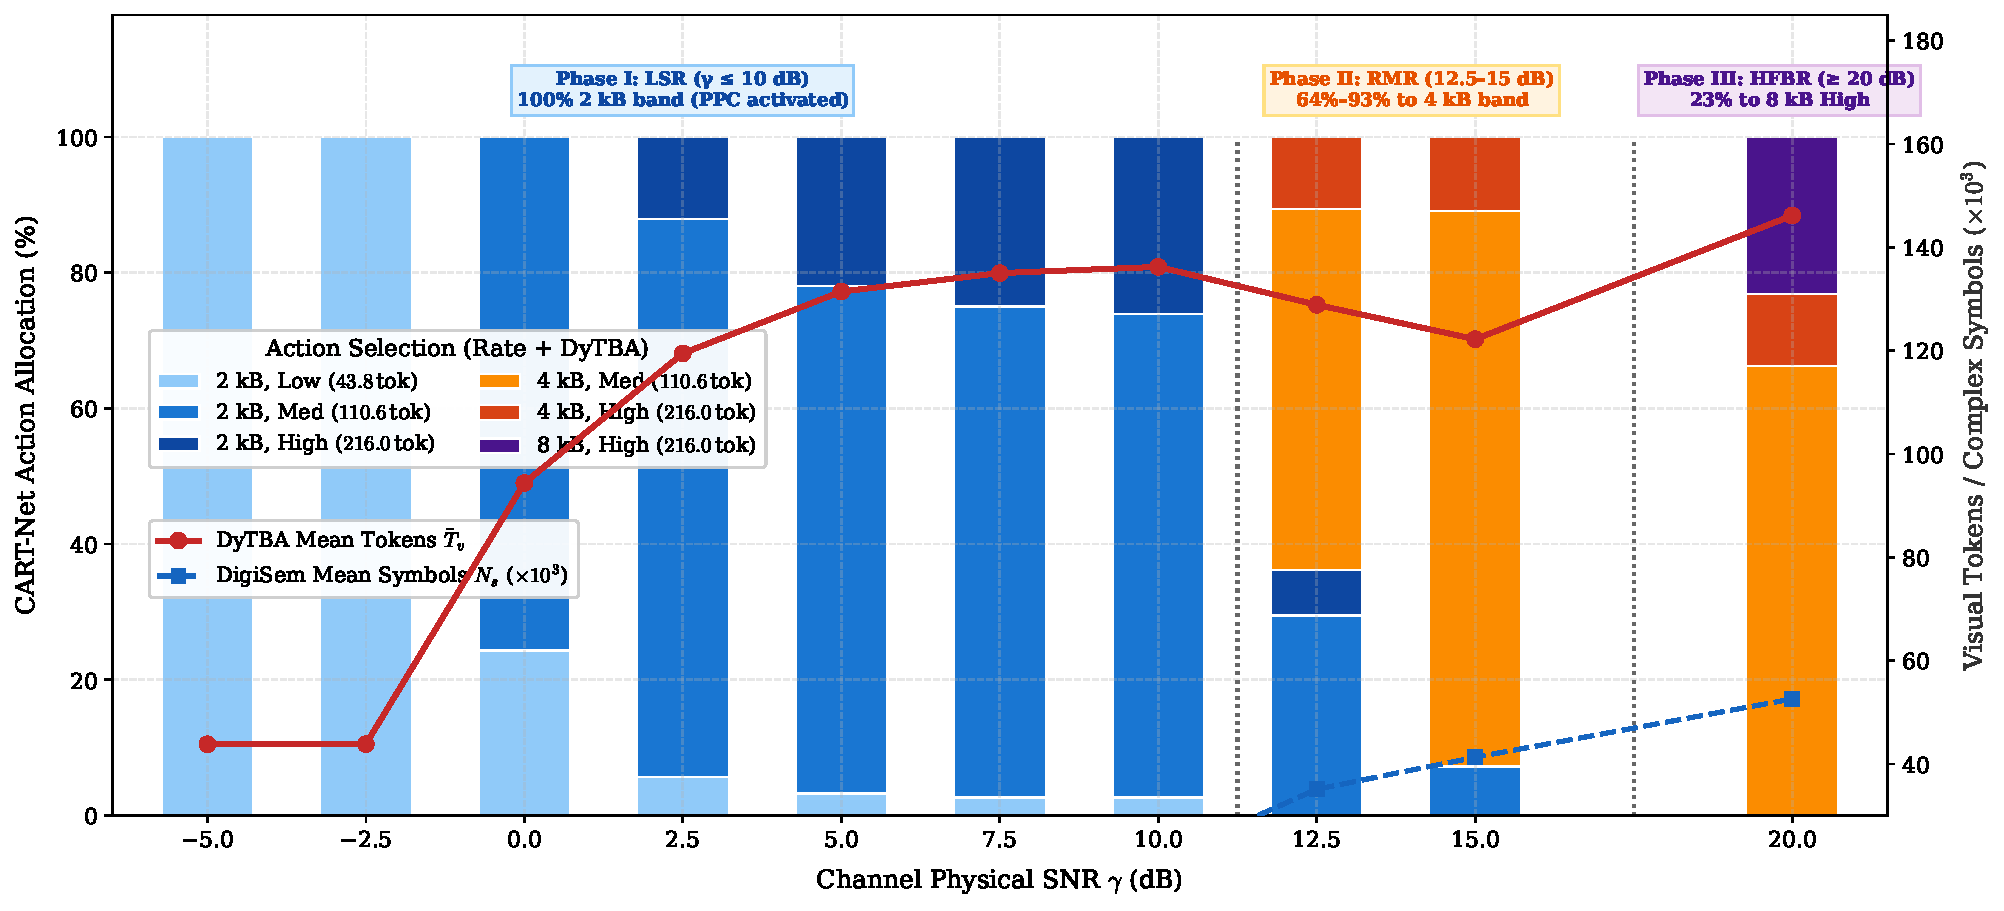
\includegraphics[width=0.96\linewidth]{figures/tgcn_publication_figures_20260922/fig2_dynamic_routing_architecture.pdf}
\caption{Overall architecture and dynamic action routing of the proposed green cross-layer semantic communication system. (a) A lightweight transmitter-side policy extracts question and image semantic cues, combines them with instantaneous channel state information (CSI) $\gamma$, and autonomously selects an action $a \in \mathcal{A}$ spanning 3 source bitrates and 3 receiver visual token budgets. (b) Empirical action routing distribution across 2,400 blind test images over Rician fading ($K=6\text{ dB}$), illustrating the emergent three-phase adaptation behavior: Link Survival ($\le 10\text{ dB}$), Rate Migration ($12.5 \sim 15\text{ dB}$), and High-Fidelity Burst ($\ge 20\text{ dB}$).}
\label{fig:framework_overview}
\end{figure*}

To bridge this gap, this paper proposes an energy-frugal, cross-layer task-oriented semantic communication framework for edge VQA, co-optimizing transmitter source coding rates and receiver visual token budgets under digital LDPC-coded Rician fading channels. As illustrated in Fig.~\ref{fig:framework_overview}, the system features a neural variational image compression engine, a digital physical layer with 3GPP LDPC coding, and an edge-deployed Qwen-VL model adapted via parameter-efficient low-rank adaptation (LoRA)~\cite{hu2021lora,dettmers2024qlora}. A lightweight cross-layer policy network observes the input question, a low-cost image preview, and instantaneous physical channel state information (CSI), dynamically allocating the source bitrate and the receiver visual token budget.

The key contributions of this paper are summarized as follows:
\begin{enumerate}
    \item \textbf{Digital-Compatible Cross-Layer SemCom Architecture}: We develop a cross-layer semantic communication architecture that integrates deep variational source coding (CompressAI hyperprior) with standardized digital channel coding ($\text{LDPC}(1020, 512)$) and an edge foundational VLM (Qwen3-VL-4B). This establishes a fully digital-compatible semantic pipeline bridging the gap between theoretical JSCC and practical wireless standards.
    \item \textbf{Dual-Mode Green Energy Formulation}: We establish rigorous end-to-end energy models incorporating both RF transmission power and edge VLM inference complexity. We formulate two operational regimes: Mode~1 (constant symbol power) and Mode~2 (constant query energy budget). We analytically and empirically demonstrate that in Mode~2, allocating compact bitrates yields up to $+3.01\text{ dB}$ and $+6.00\text{ dB}$ in physical SNR margin, effectively eliminating packet erasure under severe fading.
    \item \textbf{Channel-Aware Semantic Policy Network}: We design a lightweight, multi-branch neural policy that maps query text embeddings, image spatial features, and physical channel SNR $\gamma$ into a joint action space $\mathcal{A} = \{2\text{k}, 4\text{k}, 8\text{k}\} \times \{\text{low}, \text{medium}, \text{high}\}$. The policy autonomously exhibits a three-phase adaptation mechanism: a \emph{Link Survival Regime} ($\le 10\text{ dB}$), a \emph{Rate Migration Regime} ($12.5 \sim 15\text{ dB}$), and a \emph{High-Fidelity Burst Regime} ($\ge 20\text{ dB}$).
    \item \textbf{Large-Scale Empirical Verification}: We evaluate the framework over 2,400 independent blind test images across 10 channel SNR points ($-5\text{ dB}$ to $20\text{ dB}$) under Rician fading ($K=6\text{ dB}$) on the TDIUC benchmark. Experimental results demonstrate that under harsh fading ($\gamma = 2.5\text{ dB}$), our policy achieves $36.92\%$ accuracy, outperforming fixed 4k by $+29.92\%$ and channel-blind policies by $+27.71\%$. Furthermore, the proposed policy strictly establishes the non-dominated Pareto efficiency frontier across RF energy, system latency, and task accuracy.
\end{enumerate}

The remainder of this paper is organized as follows. Section~\ref{sec:related} reviews related work on semantic communications, vision--language models, and green edge computing. Section~\ref{sec:system} presents the system model and problem formulation under dual energy modes. Section~\ref{sec:policy} details the cross-layer policy network and its optimization. Section~\ref{sec:experiments} reports extensive empirical results, baseline comparisons, and ablation studies. Finally, Section~\ref{sec:conclusion} concludes the paper.
